\section{Ejemplos Resueltos}

¡Ahora sí viene lo bueno! Vamos a resolver problemas reales paso a paso. Presta mucha atención porque estos ejemplos te mostrarán exactamente cómo aplicar todo lo que has aprendido.

\begin{ejemplo}
\textbf{Ejemplo 1: El Edificio Misterioso}

\textbf{Enunciado:}
Un estudiante de arquitectura necesita calcular la altura de un edificio. Se para a 50 metros de la base y mide que el ángulo de elevación hacia la azotea es de 35°. ¿Cuál es la altura del edificio?

\textbf{Solución:}

\textbf{Paso 1: Identificar los datos}
\begin{itemize}
\item Distancia horizontal desde el observador al edificio: 50 m
\item Ángulo de elevación: 35°
\item Buscamos: altura del edificio
\end{itemize}

\textbf{Paso 2: Hacer un diagrama}
\begin{center}
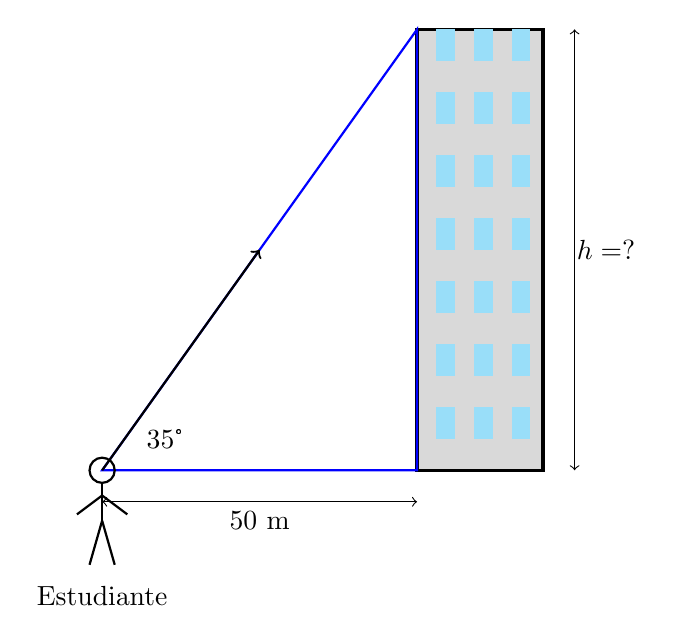
\begin{tikzpicture}[scale=0.08]
% Edificio
\fill[gray!30] (0,0) rectangle (20,70);
\draw[very thick] (0,0) -- (0,70) -- (20,70) -- (20,0) -- cycle;
% Ventanas
\foreach \x in {3,9,15} {
    \foreach \y in {5,15,25,35,45,55,65} {
        \fill[cyan!40] (\x,\y) rectangle (\x+3,\y+5);
    }
}
% Triángulo
\draw[thick, blue] (-50,0) -- (0,0) -- (0,70) -- cycle;
\draw[thick, ->] (-50,0) -- (-25,35);
\node at (-40,5) {35°};
\draw[<->] (-50,-5) -- (0,-5);
\node at (-25,-8) {50 m};
\draw[<->] (25,0) -- (25,70);
\node at (30,35) {$h = ?$};
% Persona
\draw[thick] (-50,0) circle (2);
\draw[thick] (-50,-2) -- (-50,-8);
\draw[thick] (-50,-8) -- (-52,-15);
\draw[thick] (-50,-8) -- (-48,-15);
\draw[thick] (-50,-4) -- (-54,-7);
\draw[thick] (-50,-4) -- (-46,-7);
\node at (-50,-20) {Estudiante};
\end{tikzpicture}
\end{center}

\textbf{Paso 3: Identificar qué se busca}
\begin{itemize}
\item Altura del edificio ($h$)
\item Es el cateto opuesto al ángulo de 35°
\end{itemize}

\textbf{Paso 4: Elegir la razón trigonométrica apropiada}

Tenemos:
\begin{itemize}
\item Cateto adyacente = 50 m
\item Ángulo = 35°
\item Buscamos: Cateto opuesto
\end{itemize}

¿Qué razón relaciona cateto opuesto con cateto adyacente? ¡La tangente!

$$\tan(35°) = \frac{\text{cateto opuesto}}{\text{cateto adyacente}} = \frac{h}{50}$$

\textbf{Paso 5: Resolver}
\begin{align}
\tan(35°) &= \frac{h}{50}\\
h &= 50 \cdot \tan(35°)\\
h &= 50 \cdot 0.7002\\
h &= 35.01 \text{ metros}
\end{align}

\textbf{Paso 6: Verificar}

Vamos a comprobar usando el teorema de Pitágoras. Si $h = 35.01$ m y la base es 50 m, entonces:
\begin{itemize}
\item Hipotenusa = $\sqrt{50^2 + 35.01^2} = \sqrt{2500 + 1225.7} = \sqrt{3725.7} = 61.04$ m
\end{itemize}

Ahora verificamos con seno:
$$\sin(35°) = \frac{35.01}{61.04} = 0.5736 \checkmark$$

¡Correcto! $\sin(35°) = 0.5736$

\begin{tcolorbox}[colback=solutioncolor!10, colframe=solutioncolor, title=Respuesta]
La altura del edificio es de \textbf{35.01 metros}.
\end{tcolorbox}
\end{ejemplo}

\begin{ejemplo}
\textbf{Ejemplo 2: La Rampa de Acceso Perfecta}

\textbf{Enunciado:}
En un centro comercial necesitan construir una rampa de acceso para personas con movilidad reducida. La rampa debe tener una longitud de 8 metros y formar un ángulo de 7° con el suelo (cumpliendo con las normas de accesibilidad). ¿Qué altura alcanzará la rampa y cuál será su proyección horizontal?

\textbf{Solución:}

\textbf{Paso 1: Identificar los datos}
\begin{itemize}
\item Longitud de la rampa (hipotenusa): 8 m
\item Ángulo con el suelo: 7°
\item Buscamos: altura y proyección horizontal
\end{itemize}

\textbf{Paso 2: Hacer un diagrama}
\begin{center}
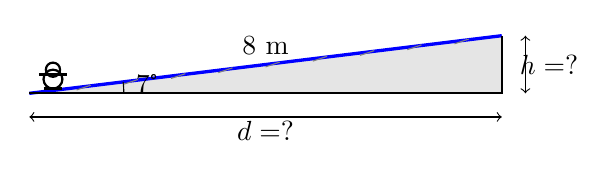
\begin{tikzpicture}[scale=0.6]
% Rampa
\fill[gray!20] (0,0) -- (10,0) -- (10,1.22) -- (0,0);
\draw[very thick, blue] (0,0) -- (10,1.22);
\draw[thick] (0,0) -- (10,0) -- (10,1.22);
% Ángulo
\draw (2,0) arc (0:7:2);
\node at (2.5,0.2) {7°};
% Medidas
\node[above,sloped] at (5,0.61) {8 m};
\draw[<->] (0,-0.5) -- (10,-0.5);
\node at (5,-0.8) {$d = ?$};
\draw[<->] (10.5,0) -- (10.5,1.22);
\node at (11,0.61) {$h = ?$};
% Textura rampa
\foreach \x in {1,2,3,4,5,6,7,8,9} {
    \draw[gray] (\x,0.122*\x-0.05) -- (\x+0.3,0.122*\x+0.05);
}
% Persona en silla de ruedas
\draw[thick] (0.5,0.3) circle (0.2);
\draw[thick] (0.3,0.1) -- (0.7,0.1);
\draw[thick] (0.2,0.4) -- (0.8,0.4);
\draw[thick] (0.5,0.5) circle (0.15);
\end{tikzpicture}
\end{center}

\textbf{Paso 3: Identificar qué se busca}
\begin{itemize}
\item Altura de la rampa ($h$) - cateto opuesto
\item Proyección horizontal ($d$) - cateto adyacente
\end{itemize}

\textbf{Paso 4: Elegir las razones trigonométricas apropiadas}

Para la altura ($h$):
$$\sin(7°) = \frac{h}{8}$$

Para la proyección horizontal ($d$):
$$\cos(7°) = \frac{d}{8}$$

\textbf{Paso 5: Resolver}

\underline{Altura de la rampa:}
\begin{align}
\sin(7°) &= \frac{h}{8}\\
h &= 8 \cdot \sin(7°)\\
h &= 8 \cdot 0.1219\\
h &= 0.98 \text{ metros}
\end{align}

\underline{Proyección horizontal:}
\begin{align}
\cos(7°) &= \frac{d}{8}\\
d &= 8 \cdot \cos(7°)\\
d &= 8 \cdot 0.9925\\
d &= 7.94 \text{ metros}
\end{align}

\textbf{Paso 6: Verificar}

Comprobemos con Pitágoras:
$$\sqrt{h^2 + d^2} = \sqrt{0.98^2 + 7.94^2} = \sqrt{0.96 + 63.04} = \sqrt{64} = 8 \text{ m} \checkmark$$

¡Perfecto! La hipotenusa es efectivamente 8 metros.

\begin{tcolorbox}[colback=solutioncolor!10, colframe=solutioncolor, title=Respuesta]
La rampa alcanzará una altura de \textbf{0.98 metros} (98 cm) y tendrá una proyección horizontal de \textbf{7.94 metros}.
\end{tcolorbox}
\end{ejemplo}

\begin{ejemplo}
\textbf{Ejemplo 3: El Terreno de Construcción}

\textbf{Enunciado:}
Un arquitecto está diseñando una casa en un terreno triangular. El terreno forma un triángulo rectángulo donde un cateto mide 15 metros y el otro cateto mide 20 metros. Necesita conocer todos los ángulos del terreno para el diseño. ¿Cuáles son las medidas de los ángulos agudos?

\textbf{Solución:}

\textbf{Paso 1: Identificar los datos}
\begin{itemize}
\item Cateto 1: 15 m
\item Cateto 2: 20 m
\item Ángulo recto: 90°
\item Buscamos: los dos ángulos agudos
\end{itemize}

\textbf{Paso 2: Hacer un diagrama}
\begin{center}
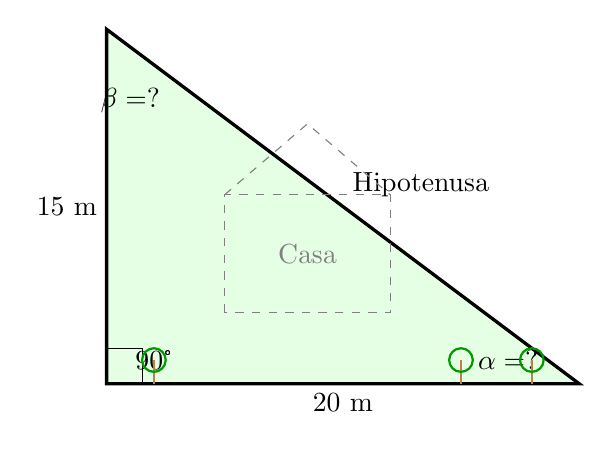
\begin{tikzpicture}[scale=0.3]
% Terreno
\fill[green!10] (0,0) -- (20,0) -- (0,15) -- cycle;
\draw[very thick] (0,0) -- (20,0) -- (0,15) -- cycle;
% Ángulo recto
\draw (0,0) rectangle (1.5,1.5);
% Medidas
\node[below] at (10,0) {20 m};
\node[left] at (0,7.5) {15 m};
\node[above right] at (10,7.5) {Hipotenusa};
% Ángulos
\node at (2,1) {90°};
\node at (17,1) {$\alpha = ?$};
\node at (1,12) {$\beta = ?$};
% Casa esquemática
\draw[dashed, gray] (5,3) rectangle (12,8);
\draw[dashed, gray] (5,8) -- (8.5,11) -- (12,8);
\node[gray] at (8.5,5.5) {Casa};
% Árboles
\foreach \x in {2,15,18} {
    \draw[brown, thick] (\x,0) -- (\x,1);
    \draw[green!60!black, thick] (\x,1) circle (0.5);
}
\end{tikzpicture}
\end{center}

\textbf{Paso 3: Identificar qué se busca}
\begin{itemize}
\item Ángulo $\alpha$ (en el vértice inferior derecho)
\item Ángulo $\beta$ (en el vértice superior)
\end{itemize}

\textbf{Paso 4: Elegir la razón trigonométrica apropiada}

Para encontrar $\alpha$, usamos la tangente:
$$\tan(\alpha) = \frac{\text{cateto opuesto}}{\text{cateto adyacente}} = \frac{15}{20}$$

\textbf{Paso 5: Resolver}

\underline{Encontrar el ángulo $\alpha$:}
\begin{align}
\tan(\alpha) &= \frac{15}{20} = 0.75\\
\alpha &= \arctan(0.75)\\
\alpha &= 36.87°
\end{align}

\underline{Encontrar el ángulo $\beta$:}

Como la suma de ángulos en un triángulo es 180°:
\begin{align}
\alpha + \beta + 90° &= 180°\\
36.87° + \beta + 90° &= 180°\\
\beta &= 180° - 90° - 36.87°\\
\beta &= 53.13°
\end{align}

\textbf{Paso 6: Verificar}

Verifiquemos usando otra razón trigonométrica:
$$\tan(\beta) = \frac{20}{15} = 1.333...$$
$$\beta = \arctan(1.333) = 53.13° \checkmark$$

También podemos verificar que:
$$\alpha + \beta + 90° = 36.87° + 53.13° + 90° = 180° \checkmark$$

\begin{tcolorbox}[colback=solutioncolor!10, colframe=solutioncolor, title=Respuesta]
Los ángulos agudos del terreno miden:
\begin{itemize}
\item Ángulo inferior derecho ($\alpha$): \textbf{36.87°}
\item Ángulo superior ($\beta$): \textbf{53.13°}
\end{itemize}
\end{tcolorbox}
\end{ejemplo}

\begin{ejemplo}
\textbf{Ejemplo 4: El Monte Chimborazo}

\textbf{Enunciado:}
Un grupo de montañistas quiere calcular la altura del Monte Chimborazo. Desde un punto en la base, miden un ángulo de elevación de 28° hacia la cima. Luego avanzan 2,500 metros en línea recta hacia la montaña y vuelven a medir, obteniendo un ángulo de elevación de 42°. ¿Cuál es la altura de la montaña desde el punto de observación?

\textbf{Solución:}

\textbf{Paso 1: Identificar los datos}
\begin{itemize}
\item Primera medición: ángulo de elevación = 28°
\item Segunda medición: ángulo de elevación = 42°
\item Distancia entre mediciones: 2,500 m
\item Buscamos: altura de la montaña ($h$)
\end{itemize}

\textbf{Paso 2: Hacer un diagrama}
\begin{center}
\begin{tikzpicture}[scale=0.0015]
% Montaña
\fill[brown!30] (0,0) -- (3000,0) -- (1500,4000) -- cycle;
\draw[very thick] (0,0) -- (1500,4000) -- (3000,0);
% Nieve en la cima
\fill[white] (1500,4000) -- (1300,3600) -- (1700,3600) -- cycle;
% Posiciones de observación
\draw[thick, blue] (-2500,0) -- (1500,4000);
\draw[thick, red] (0,0) -- (1500,4000);
% Ángulos
\draw (-2200,0) arc (0:28:300);
\node at (-2000,200) {28°};
\draw (300,0) arc (0:42:300);
\node at (500,250) {42°};
% Distancias
\draw[<->] (-2500,-300) -- (0,-300);
\node at (-1250,-500) {2,500 m};
\draw[<->] (0,-300) -- (1500,-300);
\node at (750,-500) {$x$};
% Altura
\draw[dashed] (1500,0) -- (1500,4000);
\draw[<->] (1800,0) -- (1800,4000);
\node at (2100,2000) {$h = ?$};
% Personas
\foreach \x in {-2500, 0} {
    \draw (\x,0) circle (40);
    \draw (\x,-40) -- (\x,-120);
    \draw (\x,-120) -- (\x-30,-200);
    \draw (\x,-120) -- (\x+30,-200);
}
\end{tikzpicture}
\end{center}

\textbf{Paso 3: Identificar qué se busca}
\begin{itemize}
\item Altura de la montaña ($h$)
\item Distancia horizontal desde la segunda posición hasta la base de la altura ($x$)
\end{itemize}

\textbf{Paso 4: Elegir las razones trigonométricas apropiadas}

Desde la primera posición:
$$\tan(28°) = \frac{h}{2500 + x}$$

Desde la segunda posición:
$$\tan(42°) = \frac{h}{x}$$

\textbf{Paso 5: Resolver}

De la segunda ecuación:
$$x = \frac{h}{\tan(42°)}$$

Sustituyendo en la primera ecuación:
\begin{align}
\tan(28°) &= \frac{h}{2500 + \frac{h}{\tan(42°)}}\\
\tan(28°) &= \frac{h \cdot \tan(42°)}{2500 \cdot \tan(42°) + h}\\
\tan(28°) \cdot (2500 \cdot \tan(42°) + h) &= h \cdot \tan(42°)\\
2500 \cdot \tan(28°) \cdot \tan(42°) + h \cdot \tan(28°) &= h \cdot \tan(42°)\\
2500 \cdot \tan(28°) \cdot \tan(42°) &= h \cdot \tan(42°) - h \cdot \tan(28°)\\
2500 \cdot \tan(28°) \cdot \tan(42°) &= h(\tan(42°) - \tan(28°))\\
h &= \frac{2500 \cdot \tan(28°) \cdot \tan(42°)}{\tan(42°) - \tan(28°)}\\
h &= \frac{2500 \cdot 0.5317 \cdot 0.9004}{0.9004 - 0.5317}\\
h &= \frac{1196.8}{0.3687}\\
h &= 3,246.2 \text{ metros}
\end{align}

\textbf{Paso 6: Verificar}

Calculemos $x$:
$$x = \frac{3246.2}{0.9004} = 3,604.7 \text{ m}$$

Verificación desde la primera posición:
$$\tan(28°) = \frac{3246.2}{2500 + 3604.7} = \frac{3246.2}{6104.7} = 0.5317 \checkmark$$

\begin{tcolorbox}[colback=solutioncolor!10, colframe=solutioncolor, title=Respuesta]
La altura del Monte Chimborazo desde el punto de observación es de \textbf{3,246.2 metros}.
\end{tcolorbox}
\end{ejemplo}

\begin{ejemplo}
\textbf{Ejemplo 5: El Faro y el Barco}

\textbf{Enunciado:}
Desde lo alto de un faro de 85 metros de altura, el farero observa un barco en el mar con un ángulo de depresión de 15°. ¿A qué distancia horizontal se encuentra el barco de la base del faro? ¿Cuál es la distancia directa desde la cima del faro hasta el barco?

\textbf{Solución:}

\textbf{Paso 1: Identificar los datos}
\begin{itemize}
\item Altura del faro: 85 m
\item Ángulo de depresión: 15°
\item Buscamos: distancia horizontal y distancia directa
\end{itemize}

\textbf{Paso 2: Hacer un diagrama}
\begin{center}
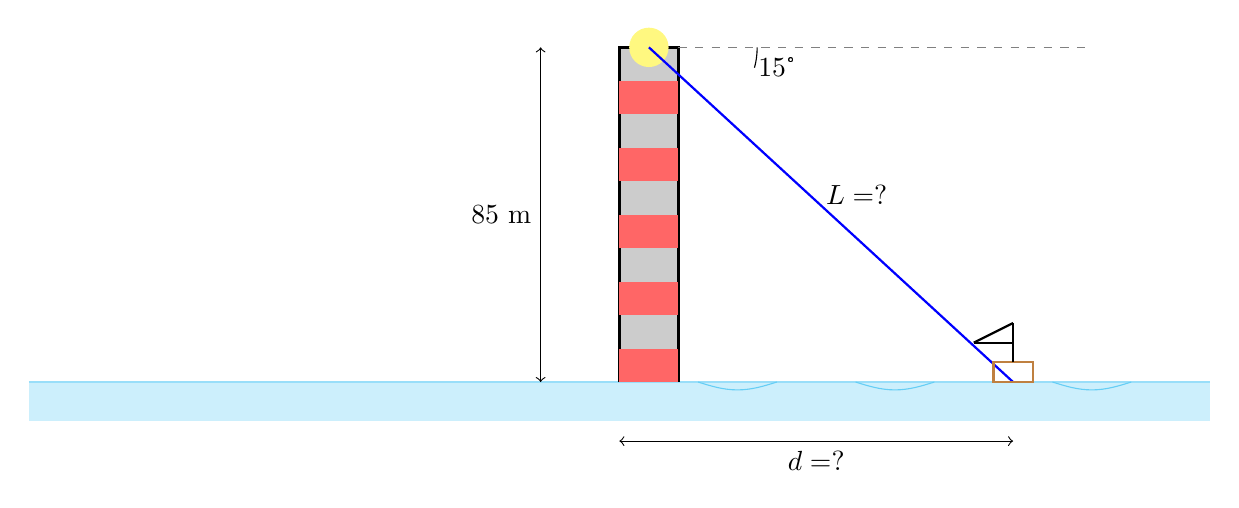
\begin{tikzpicture}[scale=0.05]
% Mar
\fill[cyan!20] (-150,0) rectangle (150,-10);
\draw[cyan!40, thick] (-150,0) -- (150,0);
% Faro
\fill[gray!40] (0,0) rectangle (15,85);
\draw[very thick] (0,0) -- (0,85) -- (15,85) -- (15,0);
% Franjas del faro
\foreach \y in {0,17,34,51,68} {
    \fill[red!60] (0,\y) rectangle (15,\y+8.5);
}
% Luz del faro
\fill[yellow!50] (7.5,85) circle (5);
% Línea horizontal de referencia
\draw[dashed, gray] (15,85) -- (120,85);
% Ángulo de depresión
\draw (35,85) arc (0:-15:20);
\node at (40,80) {15°};
% Línea de visión
\draw[thick, blue] (7.5,85) -- (100,0);
% Barco
\draw[thick, brown] (95,0) -- (105,0) -- (105,5) -- (95,5) -- cycle;
\draw[thick] (100,5) -- (100,15);
\draw[thick] (100,10) -- (90,10);
\draw[thick] (100,15) -- (90,10);
% Medidas
\draw[<->] (-20,0) -- (-20,85);
\node at (-30,42.5) {85 m};
\draw[<->] (0,-15) -- (100,-15);
\node at (50,-20) {$d = ?$};
% Distancia directa
\node[above right] at (50,42.5) {$L = ?$};
% Olas
\draw[cyan!60] (20,0) sin (30,-2) cos (40,0);
\draw[cyan!60] (60,0) sin (70,-2) cos (80,0);
\draw[cyan!60] (110,0) sin (120,-2) cos (130,0);
\end{tikzpicture}
\end{center}

\textbf{Paso 3: Identificar qué se busca}
\begin{itemize}
\item Distancia horizontal ($d$) desde la base del faro hasta el barco
\item Distancia directa ($L$) desde la cima del faro hasta el barco
\end{itemize}

\textbf{Paso 4: Elegir las razones trigonométricas apropiadas}

Nota importante: El ángulo de depresión desde la horizontal es igual al ángulo de elevación desde el barco hacia el faro (ángulos alternos internos).

Por lo tanto, trabajamos con un ángulo de 15° en el triángulo:
$$\tan(15°) = \frac{85}{d}$$

Para la distancia directa:
$$\sin(15°) = \frac{85}{L}$$

\textbf{Paso 5: Resolver}

\underline{Distancia horizontal:}
\begin{align}
\tan(15°) &= \frac{85}{d}\\
d &= \frac{85}{\tan(15°)}\\
d &= \frac{85}{0.2679}\\
d &= 317.3 \text{ metros}
\end{align}

\underline{Distancia directa:}
\begin{align}
\sin(15°) &= \frac{85}{L}\\
L &= \frac{85}{\sin(15°)}\\
L &= \frac{85}{0.2588}\\
L &= 328.4 \text{ metros}
\end{align}

\textbf{Paso 6: Verificar}

Usando el teorema de Pitágoras:
$$L = \sqrt{85^2 + 317.3^2} = \sqrt{7225 + 100679.3} = \sqrt{107904.3} = 328.5 \text{ m} \checkmark$$

La pequeña diferencia se debe al redondeo. ¡Está correcto!

\begin{tcolorbox}[colback=solutioncolor!10, colframe=solutioncolor, title=Respuesta]
\begin{itemize}
\item El barco se encuentra a \textbf{317.3 metros} de la base del faro.
\item La distancia directa desde la cima del faro hasta el barco es de \textbf{328.4 metros}.
\end{itemize}
\end{tcolorbox}
\end{ejemplo}

\begin{ejemplo}
\textbf{Ejemplo 6: Navegación en el Caribe}

\textbf{Enunciado:}
Un barco turístico sale del puerto de Cartagena y navega 120 km con rumbo N30°E (30° al este del norte). Luego cambia su rumbo a S60°E (60° al este del sur) y navega 80 km más. ¿A qué distancia en línea recta se encuentra del puerto de origen? ¿En qué dirección debe navegar para regresar directamente al puerto?

\textbf{Solución:}

\textbf{Paso 1: Identificar los datos}
\begin{itemize}
\item Primera etapa: 120 km con rumbo N30°E
\item Segunda etapa: 80 km con rumbo S60°E
\item Buscamos: distancia directa al puerto y dirección de regreso
\end{itemize}

\textbf{Paso 2: Hacer un diagrama}
\begin{center}
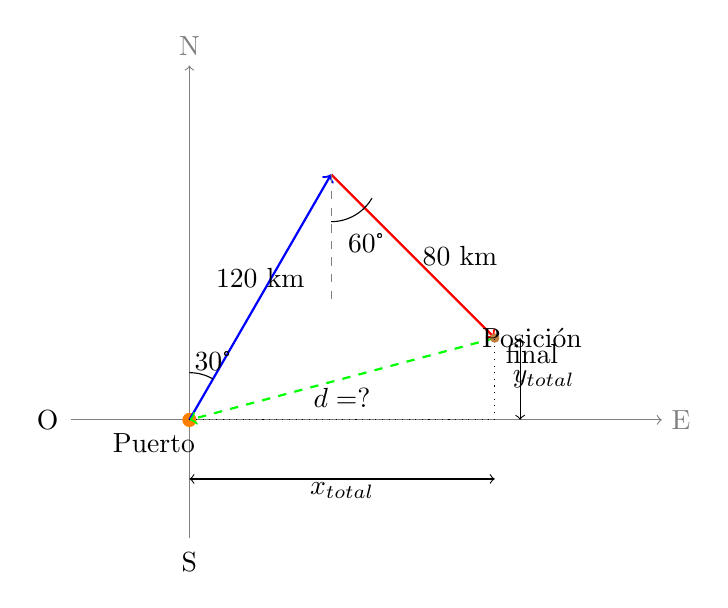
\begin{tikzpicture}[scale=0.03]
% Ejes cardinales
\draw[gray, ->] (0,-50) -- (0,150) node[above] {N};
\draw[gray, ->] (-50,0) -- (200,0) node[right] {E};
\node at (0,-60) {S};
\node at (-60,0) {O};
% Puerto
\fill[orange] (0,0) circle (3);
\node at (-15,-10) {Puerto};
% Primera etapa
\draw[thick, blue, ->] (0,0) -- (60,103.92);
\node[above] at (30,51.96) {120 km};
\draw (0,20) arc (90:60:20);
\node at (10,25) {30°};
% Segunda etapa
\draw[thick, red, ->] (60,103.92) -- (129.28,34.64);
\node[right] at (94.64,69.28) {80 km};
% Ángulo de la segunda etapa
\draw[dashed, gray] (60,103.92) -- (60,50);
\draw (60,83.92) arc (270:330:20);
\node at (75,75) {60°};
% Distancia de regreso
\draw[thick, green, dashed, ->] (129.28,34.64) -- (0,0);
\node[below] at (64.64,17.32) {$d = ?$};
% Barco
\fill[brown] (129.28,34.64) circle (2);
% Posición final
\node at (145,34.64) {Posición};
\node at (145,28) {final};
% Componentes
\draw[dotted] (0,0) -- (129.28,0) -- (129.28,34.64);
\draw[<->] (0,-25) -- (129.28,-25);
\node at (64.64,-30) {$x_{total}$};
\draw[<->] (140,0) -- (140,34.64);
\node at (150,17.32) {$y_{total}$};
\end{tikzpicture}
\end{center}

\textbf{Paso 3: Descomponer los movimientos en componentes}

\underline{Primera etapa (N30°E):}
\begin{itemize}
\item Componente Este: $x_1 = 120 \cdot \sin(30°) = 120 \cdot 0.5 = 60$ km
\item Componente Norte: $y_1 = 120 \cdot \cos(30°) = 120 \cdot 0.866 = 103.92$ km
\end{itemize}

\underline{Segunda etapa (S60°E):}
\begin{itemize}
\item Componente Este: $x_2 = 80 \cdot \cos(60°) = 80 \cdot 0.866 = 69.28$ km
\item Componente Sur: $y_2 = -80 \cdot \sin(60°) = -80 \cdot 0.5 = -69.28$ km
\end{itemize}

\textbf{Paso 4: Calcular la posición final}

\underline{Posición total:}
\begin{itemize}
\item $x_{total} = x_1 + x_2 = 60 + 69.28 = 129.28$ km Este
\item $y_{total} = y_1 + y_2 = 103.92 - 69.28 = 34.64$ km Norte
\end{itemize}

\textbf{Paso 5: Calcular la distancia directa al puerto}

Usando el teorema de Pitágoras:
\begin{align}
d &= \sqrt{x_{total}^2 + y_{total}^2}\\
d &= \sqrt{129.28^2 + 34.64^2}\\
d &= \sqrt{16713.3 + 1199.9}\\
d &= \sqrt{17913.2}\\
d &= 133.8 \text{ km}
\end{align}

\textbf{Paso 6: Calcular la dirección de regreso}

El ángulo respecto al norte:
\begin{align}
\tan(\theta) &= \frac{x_{total}}{y_{total}} = \frac{129.28}{34.64} = 3.733\\
\theta &= \arctan(3.733) = 75.0°
\end{align}

Para regresar, el barco debe navegar en dirección opuesta:
Rumbo de regreso = S75°O (75° al oeste del sur)

\begin{tcolorbox}[colback=solutioncolor!10, colframe=solutioncolor, title=Respuesta]
\begin{itemize}
\item El barco se encuentra a \textbf{133.8 km} del puerto en línea recta.
\item Para regresar directamente, debe navegar con rumbo \textbf{S75°O}.
\end{itemize}
\end{tcolorbox}
\end{ejemplo}

\begin{ejemplo}
\textbf{Ejemplo 7: Midiendo el Ancho del Río Amazonas}

\textbf{Enunciado:}
Un equipo de topógrafos necesita medir el ancho de una sección del río Amazonas sin cruzarlo. Desde un punto A en una orilla, identifican un árbol notable (punto B) en la orilla opuesta. Luego caminan 150 metros paralelos a la orilla hasta un punto C. Desde C, miden que el ángulo ACB es de 52°. Desde A, el ángulo CAB es de 38°. ¿Cuál es el ancho del río?

\textbf{Solución:}

\textbf{Paso 1: Identificar los datos}
\begin{itemize}
\item Distancia AC (paralela a la orilla): 150 m
\item Ángulo en C (ACB): 52°
\item Ángulo en A (CAB): 38°
\item Buscamos: ancho del río (distancia perpendicular de A a la orilla opuesta)
\end{itemize}

\textbf{Paso 2: Hacer un diagrama}
\begin{center}
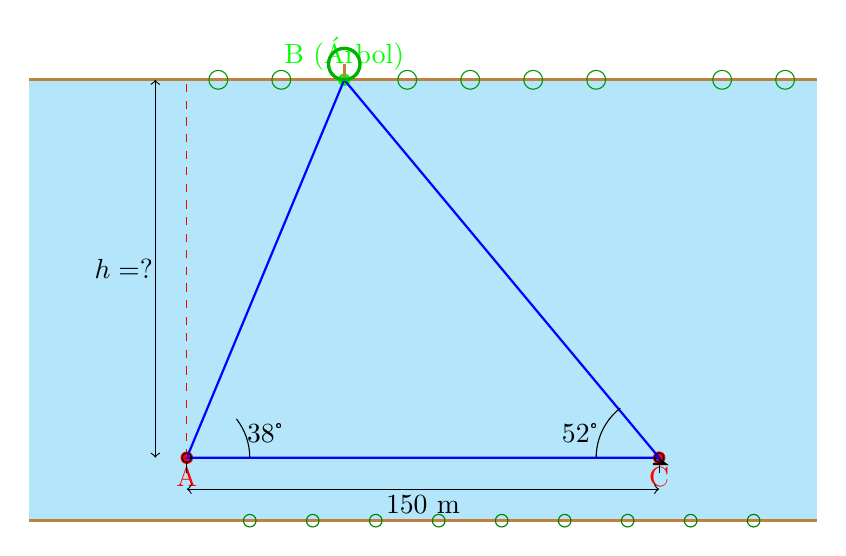
\begin{tikzpicture}[scale=0.04]
% Río
\fill[cyan!30] (-50,-20) rectangle (200,120);
% Orillas
\draw[very thick, brown] (-50,-20) -- (200,-20);
\draw[very thick, brown] (-50,120) -- (200,120);
% Puntos
\fill[red] (0,0) circle (2) node[below] {A};
\fill[red] (150,0) circle (2) node[below] {C};
\fill[green] (50,120) circle (2) node[above] {B (Árbol)};
% Triángulo
\draw[thick, blue] (0,0) -- (150,0) -- (50,120) -- cycle;
% Ángulos
\draw (20,0) arc (0:38:20);
\node at (25,8) {38°};
\draw (130,0) arc (180:128:20);
\node at (125,8) {52°};
% Distancia AC
\draw[<->] (0,-10) -- (150,-10);
\node at (75,-15) {150 m};
% Ancho del río
\draw[dashed, red] (0,0) -- (0,120);
\draw[<->] (-10,0) -- (-10,120);
\node at (-20,60) {$h = ?$};
% Vegetación
\foreach \x in {10,30,70,90,110,130,170,190} {
    \draw[green!60!black] (\x,120) circle (3);
}
\foreach \x in {20,40,60,80,100,120,140,160,180} {
    \draw[green!50!black] (\x,-20) circle (2);
}
% Árbol notable en B
\draw[brown, very thick] (50,120) -- (50,125);
\draw[green!70!black, very thick] (50,125) circle (5);
% Topógrafos
\draw (0,0) circle (1.5);
\draw (0,-1.5) -- (0,-5);
\draw (150,0) circle (1.5);
\draw (150,-1.5) -- (150,-5);
% Teodolito
\draw[thick] (148,-2) -- (152,-2) -- (150,-0.5);
\end{tikzpicture}
\end{center}

\textbf{Paso 3: Calcular el ángulo en B}

La suma de ángulos en un triángulo es 180°:
\begin{align}
\angle ABC &= 180° - 38° - 52°\\
\angle ABC &= 90°
\end{align}

¡Interesante! El triángulo ABC resulta ser rectángulo con el ángulo recto en B.

\textbf{Paso 4: Aplicar la ley de senos}

En cualquier triángulo:
$$\frac{a}{\sin A} = \frac{b}{\sin B} = \frac{c}{\sin C}$$

Donde:
\begin{itemize}
\item $BC$ es opuesto al ángulo A (38°)
\item $AB$ es opuesto al ángulo C (52°)
\item $AC = 150$ m es opuesto al ángulo B (90°)
\end{itemize}

\textbf{Paso 5: Calcular AB (distancia de A al árbol)}

$$\frac{AB}{\sin(52°)} = \frac{150}{\sin(90°)}$$

$$AB = \frac{150 \cdot \sin(52°)}{\sin(90°)} = \frac{150 \cdot 0.788}{1} = 118.2 \text{ m}$$

\textbf{Paso 6: Calcular el ancho del río}

El ancho del río es la altura del triángulo desde A perpendicular a la orilla opuesta.

Como el triángulo es rectángulo en B, y necesitamos la altura desde A:

Usando trigonometría en el triángulo:
$$h = AB \cdot \sin(38°) = 118.2 \cdot 0.616 = 72.8 \text{ m}$$

Verificación alternativa:
$$h = AC \cdot \sin(52°) \cdot \sin(38°) = 150 \cdot 0.788 \cdot 0.616 = 72.8 \text{ m} \checkmark$$

\begin{tcolorbox}[colback=solutioncolor!10, colframe=solutioncolor, title=Respuesta]
El ancho del río Amazonas en esta sección es de \textbf{72.8 metros}.
\end{tcolorbox}
\end{ejemplo}

\section{Ejercicios Inversos: Creatividad y Diseño}

¡Ahora es tu turno de ser el ingeniero! En estos ejercicios, TÚ crearás los problemas y los resolverás. Es como cuando un arquitecto primero imagina un edificio y luego hace los planos.

\begin{ejercicio}
\textbf{Ejercicio Inverso 1: El Arquitecto de Alturas}

Diseña una situación real donde necesites usar un ángulo de elevación de exactamente 30° para calcular la altura de un objeto. Tu situación debe incluir:
\begin{itemize}
\item Un contexto realista (edificio, monumento, árbol, etc.)
\item Una distancia horizontal específica
\item El proceso de medición
\end{itemize}

Especifica todos los datos necesarios y resuelve tu propio problema.

\textbf{Pistas:}
\begin{itemize}
\item Recuerda que $\tan(30°) = \frac{1}{\sqrt{3}} \approx 0.577$
\item Elige una distancia que haga los cálculos interesantes
\item Piensa en situaciones donde realmente se use este método
\end{itemize}

\textbf{Espacio para tu diseño:}
\vspace{5cm}
\end{ejercicio}

\begin{solucion}
\textbf{Solución sugerida para Ejercicio Inverso 1:}

\textbf{Situación diseñada:} La Torre del Reloj del Campus

Un estudiante de ingeniería quiere medir la altura de la torre del reloj de su universidad. Se coloca a 50 metros de la base de la torre y mide un ángulo de elevación de 30° hacia la punta del reloj.

\textbf{Datos del problema:}
\begin{itemize}
\item Distancia horizontal: 50 m
\item Ángulo de elevación: 30°
\item Altura del observador: 1.70 m (a nivel de los ojos)
\end{itemize}

\textbf{Solución:}

\begin{center}
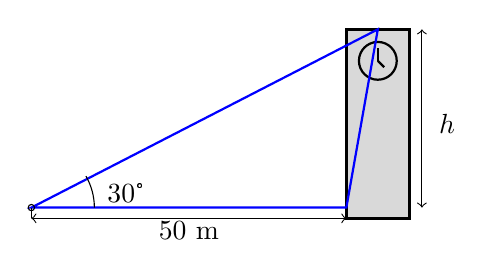
\begin{tikzpicture}[scale=0.08]
% Torre
\fill[gray!30] (0,0) rectangle (10,30);
\draw[very thick] (0,0) -- (0,30) -- (10,30) -- (10,0) -- cycle;
% Reloj
\draw[thick] (5,25) circle (3);
\draw[thick] (5,25) -- (5,27);
\draw[thick] (5,25) -- (6,24);
% Triángulo
\draw[thick, blue] (-50,1.7) -- (0,1.7) -- (5,30) -- cycle;
% Ángulo
\draw (-40,1.7) arc (0:30:10);
\node at (-35,4) {30°};
% Medidas
\draw[<->] (-50,0) -- (0,0);
\node at (-25,-2) {50 m};
\draw[<->] (12,1.7) -- (12,30);
\node at (16,15) {$h$};
% Persona
\draw (-50,0) -- (-50,1.7);
\draw (-50,1.7) circle (0.5);
\end{tikzpicture}
\end{center}

Cálculo de la altura sobre el nivel de los ojos:
$$h = 50 \cdot \tan(30°) = 50 \cdot \frac{1}{\sqrt{3}} = \frac{50}{\sqrt{3}} = \frac{50\sqrt{3}}{3} = 28.87 \text{ m}$$

Altura total de la torre:
$$H_{total} = 28.87 + 1.70 = 30.57 \text{ m}$$

\textbf{Respuesta:} La torre del reloj mide 30.57 metros de altura.
\end{solucion}

\begin{ejercicio}
\textbf{Ejercicio Inverso 2: El Topógrafo Creativo}

Crea un método para medir el ancho de un río usando DOS triángulos rectángulos. Tu método debe:
\begin{itemize}
\item Usar al menos dos posiciones de observación
\item Incluir ángulos que puedas medir con un teodolito
\item No requerir cruzar el río
\end{itemize}

Dibuja tu diseño y explica paso a paso cómo tomarías las medidas. Luego resuelve con datos específicos que tú elijas.

\textbf{Pistas:}
\begin{itemize}
\item Piensa en formar triángulos que compartan algún lado
\item Los ángulos de 45°, 30° y 60° son fáciles de trabajar
\item Considera usar puntos de referencia en ambas orillas
\end{itemize}

\textbf{Espacio para tu diseño:}
\vspace{5cm}
\end{ejercicio}

\begin{solucion}
\textbf{Solución sugerida para Ejercicio Inverso 2:}

\textbf{Método de los dos triángulos perpendiculares:}

\begin{center}
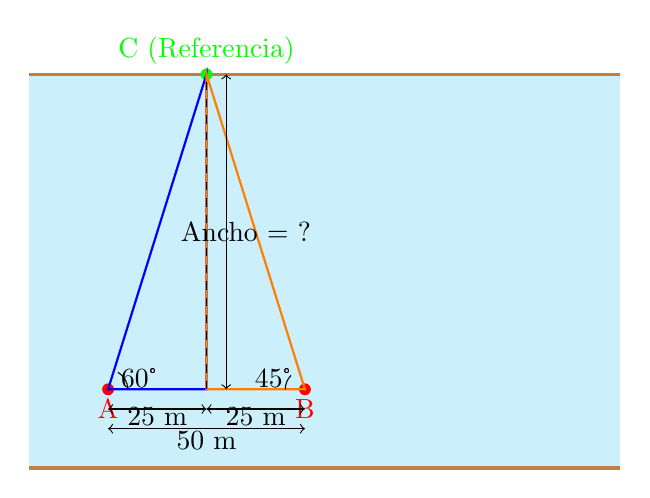
\begin{tikzpicture}[scale=0.05]
% Río
\fill[cyan!20] (0,-20) rectangle (150,80);
% Orillas
\draw[very thick, brown] (0,-20) -- (150,-20);
\draw[very thick, brown] (0,80) -- (150,80);
% Puntos de observación
\fill[red] (20,0) circle (1.5) node[below] {A};
\fill[red] (70,0) circle (1.5) node[below] {B};
\fill[green] (45,80) circle (1.5) node[above] {C (Referencia)};
% Triángulos
\draw[thick, blue] (20,0) -- (45,80) -- (45,0) -- cycle;
\draw[thick, orange] (70,0) -- (45,80) -- (45,0) -- cycle;
% Ángulos
\draw (25,0) arc (0:60:5);
\node at (28,3) {60°};
\draw (65,0) arc (180:135:5);
\node at (62,3) {45°};
% Medidas
\draw[<->] (20,-10) -- (70,-10);
\node at (45,-13) {50 m};
\draw[<->] (20,-5) -- (45,-5);
\node at (32.5,-7) {25 m};
\draw[<->] (45,-5) -- (70,-5);
\node at (57.5,-7) {25 m};
% Ancho del río
\draw[dashed] (45,0) -- (45,80);
\draw[<->] (50,0) -- (50,80);
\node at (55,40) {Ancho = ?};
\end{tikzpicture}
\end{center}

\textbf{Procedimiento:}
1. Marcar punto A en nuestra orilla
2. Identificar punto de referencia C en la orilla opuesta
3. Medir ángulo CAD = 60°
4. Caminar 50 m paralelo a la orilla hasta punto B
5. Medir ángulo CBD = 45°

\textbf{Datos elegidos:}
\begin{itemize}
\item Distancia AB = 50 m
\item Ángulo en A = 60°
\item Ángulo en B = 45°
\end{itemize}

\textbf{Resolución:}

Desde el triángulo rectángulo en A:
$$\tan(60°) = \frac{h}{x}$$
$$h = x \cdot \sqrt{3}$$

Desde el triángulo rectángulo en B:
$$\tan(45°) = \frac{h}{50-x}$$
$$h = 50 - x$$

Igualando:
$$x\sqrt{3} = 50 - x$$
$$x\sqrt{3} + x = 50$$
$$x(\sqrt{3} + 1) = 50$$
$$x = \frac{50}{\sqrt{3} + 1} = \frac{50(\sqrt{3} - 1)}{2} = 18.3 \text{ m}$$

Por lo tanto:
$$h = 50 - 18.3 = 31.7 \text{ m}$$

\textbf{Respuesta:} El ancho del río es de 31.7 metros.
\end{solucion}

\begin{ejercicio}
\textbf{Ejercicio Inverso 3: El Navegante Estratégico}

Diseña una ruta de navegación para un barco turístico que debe:
\begin{itemize}
\item Salir del puerto
\item Hacer DOS cambios de dirección (usa ángulos de 45° y 60°)
\item Visitar una isla y luego regresar al puerto
\end{itemize}

Calcula:
- Las distancias totales recorridas en cada tramo
- La distancia directa desde la isla al puerto
- El rumbo de regreso directo

\textbf{Pistas:}
\begin{itemize}
\item Usa un sistema de coordenadas con el puerto en el origen
\item Los rumbos se miden desde el norte en sentido horario
\item Descompón cada movimiento en componentes N-S y E-O
\end{itemize}

\textbf{Espacio para tu diseño:}
\vspace{5cm}
\end{ejercicio}

\begin{solucion}
\textbf{Solución sugerida para Ejercicio Inverso 3:}

\textbf{Ruta diseñada:} Tour Isla del Tesoro

\begin{center}
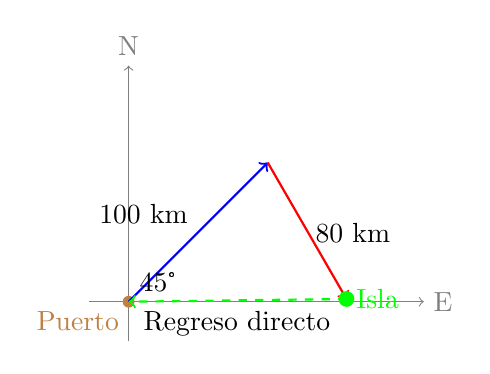
\begin{tikzpicture}[scale=0.025]
% Ejes
\draw[gray, ->] (0,-20) -- (0,120) node[above] {N};
\draw[gray, ->] (-20,0) -- (150,0) node[right] {E};
% Puerto
\fill[brown] (0,0) circle (3) node[below left] {Puerto};
% Tramo 1: N45°E, 100 km
\draw[thick, blue, ->] (0,0) -- (70.7,70.7);
\node[above left] at (35,35) {100 km};
\node at (15,10) {45°};
% Tramo 2: E60°S, 80 km
\draw[thick, red, ->] (70.7,70.7) -- (110.7,1.42);
\node[right] at (90,35) {80 km};
% Isla
\fill[green] (110.7,1.42) circle (4) node[right] {Isla};
% Regreso directo
\draw[thick, green, dashed, ->] (110.7,1.42) -- (0,0);
\node[below] at (55,0) {Regreso directo};
\end{tikzpicture}
\end{center}

\textbf{Análisis de la ruta:}

\underline{Tramo 1: Puerto a punto intermedio}
\begin{itemize}
\item Rumbo: N45°E
\item Distancia: 100 km
\item Componente Este: $100 \sin(45°) = 70.7$ km
\item Componente Norte: $100 \cos(45°) = 70.7$ km
\item Posición: (70.7, 70.7)
\end{itemize}

\underline{Tramo 2: Punto intermedio a isla}
\begin{itemize}
\item Rumbo: S60°E (equivale a 150° desde el norte)
\item Distancia: 80 km
\item Componente Este: $80 \sin(60°) = 69.3$ km
\item Componente Sur: $80 \cos(60°) = 40$ km
\item Cambio de posición: (40, -69.3)
\item Posición final de la isla: (110.7, 1.4)
\end{itemize}

\underline{Cálculo del regreso directo:}

Distancia directa:
$$d = \sqrt{110.7^2 + 1.4^2} = \sqrt{12254.5 + 2.0} = 110.7 \text{ km}$$

Ángulo respecto al norte:
$$\theta = \arctan\left(\frac{110.7}{1.4}\right) = 89.3°$$

Rumbo de regreso: S89.3°O (casi directamente hacia el oeste)

\textbf{Resumen:}
\begin{itemize}
\item Distancia total ida: 180 km
\item Distancia regreso directo: 110.7 km
\item Ahorro de distancia: 69.3 km
\item Rumbo de regreso: S89.3°O
\end{itemize}
\end{solucion}

\begin{ejercicio}
\textbf{Ejercicio Inverso 4: El Detective de Ángulos}

Te dan las tres medidas de los lados de un triángulo rectángulo: 5 cm, 12 cm y 13 cm.

Tu misión:
\begin{itemize}
\item Verifica que es un triángulo rectángulo
\item SIN USAR CALCULADORA, encuentra los valores exactos de seno, coseno y tangente de cada ángulo agudo
\item Estima los ángulos usando los valores notables que conoces (30°, 45°, 60°)
\item Crea una aplicación práctica donde usarías este triángulo
\end{itemize}

\textbf{Pistas:}
\begin{itemize}
\item Este es un triángulo pitagórico famoso
\item Las razones trigonométricas serán fracciones simples
\item Compara con los valores de ángulos notables para estimar
\end{itemize}

\textbf{Espacio para tu trabajo:}
\vspace{5cm}
\end{ejercicio}

\begin{solucion}
\textbf{Solución sugerida para Ejercicio Inverso 4:}

\textbf{Verificación del triángulo rectángulo:}
$$5^2 + 12^2 = 25 + 144 = 169 = 13^2 \checkmark$$

Sí es un triángulo rectángulo con catetos 5 y 12, e hipotenusa 13.

\begin{center}
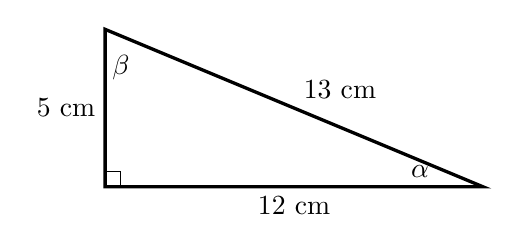
\begin{tikzpicture}[scale=0.4]
\draw[very thick] (0,0) -- (12,0) -- (0,5) -- cycle;
\draw (0,0) rectangle (0.5,0.5);
\node[below] at (6,0) {12 cm};
\node[left] at (0,2.5) {5 cm};
\node[above right] at (6,2.5) {13 cm};
\node at (10,0.5) {$\alpha$};
\node at (0.5,3.8) {$\beta$};
\end{tikzpicture}
\end{center}

\textbf{Cálculo de razones trigonométricas:}

Para el ángulo $\alpha$ (opuesto al lado de 5 cm):
\begin{itemize}
\item $\sin(\alpha) = \frac{5}{13}$
\item $\cos(\alpha) = \frac{12}{13}$
\item $\tan(\alpha) = \frac{5}{12}$
\end{itemize}

Para el ángulo $\beta$ (opuesto al lado de 12 cm):
\begin{itemize}
\item $\sin(\beta) = \frac{12}{13}$
\item $\cos(\beta) = \frac{5}{13}$
\item $\tan(\beta) = \frac{12}{5} = 2.4$
\end{itemize}

\textbf{Estimación de ángulos:}

Para $\alpha$:
- $\tan(\alpha) = \frac{5}{12} \approx 0.417$
- Sabemos que $\tan(30°) \approx 0.577$
- Por lo tanto, $\alpha < 30°$
- Estimación: $\alpha \approx 23°$

Para $\beta$:
- $\tan(\beta) = 2.4$
- Sabemos que $\tan(60°) \approx 1.732$
- Por lo tanto, $\beta > 60°$
- Estimación: $\beta \approx 67°$

Verificación: $23° + 67° + 90° = 180° \checkmark$

\textbf{Aplicación práctica: Rampa de carga}

Un camión necesita una rampa para cargar mercancía. Si la altura de la plataforma es 5 metros y disponemos de 12 metros horizontales, necesitaremos una rampa de 13 metros. El ángulo de inclinación será de aproximadamente 23°, que es seguro para el tránsito de montacargas.
\end{solucion}

\begin{ejercicio}
\textbf{Ejercicio Inverso 5: El Ingeniero de Rampas}

Las normas de accesibilidad establecen que una rampa para silla de ruedas no debe tener una pendiente mayor al 8.33\% (que significa subir 8.33 cm por cada 100 cm horizontales).

Tu tarea:
\begin{itemize}
\item Convierte este porcentaje a un ángulo
\item Si necesitas salvar una altura de 1.2 metros, calcula la longitud mínima de la rampa
\item Diseña un sistema de rampa con descansos si la longitud es muy grande
\item Verifica que tu diseño cumple con las normas
\end{itemize}

\textbf{Pistas:}
\begin{itemize}
\item Pendiente = $\tan(\theta) = \frac{\text{altura}}{\text{distancia horizontal}}$
\item 8.33\% = 0.0833 = 8.33/100
\item Las rampas muy largas necesitan descansos cada cierta distancia
\end{itemize}

\textbf{Espacio para tu diseño:}
\vspace{5cm}
\end{ejercicio}

\begin{solucion}
\textbf{Solución sugerida para Ejercicio Inverso 5:}

\textbf{Conversión de pendiente a ángulo:}

Pendiente = 8.33\% = 0.0833
$$\tan(\theta) = 0.0833$$
$$\theta = \arctan(0.0833) = 4.76°$$

\textbf{Cálculo de la rampa para 1.2 m de altura:}

\begin{center}
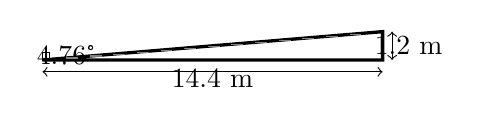
\begin{tikzpicture}[scale=0.3]
% Rampa simple
\draw[very thick] (0,0) -- (14.4,0) -- (14.4,1.2) -- (0,0);
\draw (0,0) rectangle (0.3,0.3);
\node at (1,0.2) {4.76°};
\draw[<->] (0,-0.5) -- (14.4,-0.5);
\node at (7.2,-0.8) {14.4 m};
\draw[<->] (14.8,0) -- (14.8,1.2);
\node at (15.5,0.6) {1.2 m};
% Rampa con textura
\foreach \x in {1,2,...,13} {
    \draw[gray] (\x,0.0833*\x) -- (\x+0.5,0.0833*\x);
}
\end{tikzpicture}
\end{center}

Distancia horizontal mínima:
$$d = \frac{h}{\tan(\theta)} = \frac{1.2}{0.0833} = 14.4 \text{ m}$$

Longitud de la rampa:
$$L = \frac{h}{\sin(\theta)} = \frac{1.2}{\sin(4.76°)} = \frac{1.2}{0.083} = 14.46 \text{ m}$$

\textbf{Problema:} ¡14.4 metros es demasiado largo para una rampa continua!

\textbf{Solución con descansos:}

Dividir en 3 tramos de 0.4 m de altura cada uno:

\begin{center}
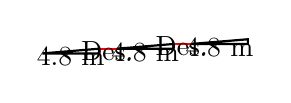
\begin{tikzpicture}[scale=0.15]
% Tramo 1
\draw[thick] (0,0) -- (4.8,0) -- (4.8,0.4) -- (0,0);
% Descanso 1
\draw[thick, red] (4.8,0.4) -- (6.3,0.4);
% Tramo 2
\draw[thick] (6.3,0.4) -- (11.1,0.4) -- (11.1,0.8) -- (6.3,0.4);
% Descanso 2
\draw[thick, red] (11.1,0.8) -- (12.6,0.8);
% Tramo 3
\draw[thick] (12.6,0.8) -- (17.4,0.8) -- (17.4,1.2) -- (12.6,0.8);
% Etiquetas
\node at (2.4,-0.3) {4.8 m};
\node at (5.5,0.2) {Des.};
\node at (8.7,0.1) {4.8 m};
\node at (11.8,0.6) {Des.};
\node at (15,0.5) {4.8 m};
\end{tikzpicture}
\end{center}

\textbf{Diseño final:}
\begin{itemize}
\item 3 tramos de rampa de 4.8 m cada uno
\item 2 descansos de 1.5 m
\item Longitud total: $3 \times 4.8 + 2 \times 1.5 = 17.4$ m
\item Cada tramo sube 0.4 m (40 cm)
\item Pendiente verificada: $\frac{0.4}{4.8} = 0.0833 = 8.33\%$ ✓
\end{itemize}

\textbf{Ventajas del diseño:}
- Cumple con las normas de accesibilidad
- Proporciona áreas de descanso
- Es más seguro y cómodo para los usuarios
\end{solucion}

\section*{¡Felicitaciones!}

Has completado los ejemplos resueltos y los ejercicios inversos. Ahora tienes todas las herramientas para resolver problemas reales con triángulos rectángulos.

Recuerda:
\begin{itemize}
\item Siempre hacer un diagrama claro
\item Identificar qué datos tienes y qué buscas
\item Elegir la razón trigonométrica correcta
\item Verificar tus respuestas
\item ¡La práctica hace al maestro!
\end{itemize}

Los ejercicios inversos te han enseñado algo muy importante: no solo puedes resolver problemas, ¡también puedes crearlos! Esto es lo que hacen los ingenieros, arquitectos y científicos todos los días: diseñan soluciones para problemas reales.